\documentclass[tikz,border=1mm]{standalone}

\usepackage{amsmath}
\usepackage{graphicx}
\renewcommand\familydefault{\sfdefault} 
\usepackage[T1]{fontenc}

\usetikzlibrary{arrows,shapes,calc,math,decorations.fractals,patterns,backgrounds,decorations.markings}
\tikzset{every picture/.style={/utils/exec={\sffamily}}}
\tikzset{point/.style={fill,circle,inner sep=1.5pt}}
\tikzset{vel/.style={-triangle 45,blue!50!black,line width=1pt}}
\tikzset{acc/.style={-triangle 45,red,line width=1pt}}
\tikzset{myarrow/.style={decoration={markings,mark=at position 1 with %
    {\arrow[scale=3,>=stealth]{>}}},postaction={decorate}}}

\begin{document}

% % Pendulum
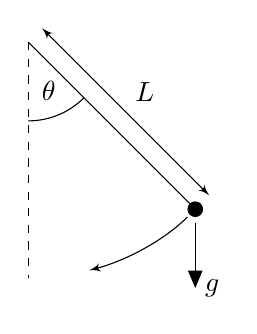
\begin{tikzpicture}[auto]
    \draw (0, 0) -- (315:3) node [fill, circle, inner sep=2pt] (1) {};
    \draw [dashed] (0, 0) -- (0, -3);
    \draw (315:1) arc (315:270:1);
    \draw [-triangle 45,shorten <= 2pt] (1) -- ++(0, -1) node [right] {$g$};
    \draw [latex'-latex'] (45:0.25) -- node {$L$} ++(315:3);
    \node at (293:0.67) {$\theta$};
    \draw [-latex', shorten <= 4pt] (1) arc (315:285:3);
\end{tikzpicture}

% % Interval of absolute stability
% \begin{tikzpicture}
%     \fill [white] (-6, -3) rectangle (4, 3);
%     \draw [fill=blue!20!white,line width=1pt] (-1.5, 0) circle (1.5cm);
%     \draw [-stealth'] (-4, 0) -- (2, 0) node [below] {$\operatorname{Re}(z)$};
%     \draw [-stealth'] (0, -2.5) -- (0, 2.5) node [left] {$\operatorname{Im}(z)$};
%     \draw [latex'-latex', shorten >= 2pt, shorten <= 2pt] (-3, -0.25) -- node [below,text width=2cm,align=center] {stability interval} (0, -0.25);
%     \node at (-4, 2) (1) {stability region};
%     \draw [-latex'] (1) -- ($(-1.5,0)+(135:1.5)$);
%     \node at (-1.5, 0.5) {$|R(z)| < 1$};
%     \node at (1.5, 1.5) {$|R(z)| > 1$};
% \end{tikzpicture}

% % Gram-Schmidt
% \begin{tikzpicture}
%     \draw [-triangle 45] (0, 0) -- (15:4) node [below,anchor=north west] {$\mathbf{u}_1 = \mathbf{a}_1$};
%     \draw [-triangle 45] (0, 0) -- (105:3) node [left] {$\mathbf{u}_2$};
%     \draw [-triangle 45] (0, 0) -- (45:2.5) coordinate (1) node [below, anchor=north west] {$\mathbf{a}_2$};
%     \draw [-triangle 45] (1) -- ++(195:2.2) node [pos=0.5,rotate=15, above] {$-\operatorname{proj}_{\mathbf{u}_1} \mathbf{a}_2$};
%     \draw [-triangle 45] (0, 0) -- (15:2.2) node [pos=0.5,rotate=15,below] {$\operatorname{proj}_{\mathbf{u}_1} \mathbf{a}_2$};
% \end{tikzpicture}

% Householder
% \begin{tikzpicture}
%     \draw [-triangle 45] (0, 0) -- (45:3) node [pos=0.67, below right] {$\mathbf{x}$};
%     \draw [-triangle 45] (0, 0) -- (0:3) node [pos=0.67,below] {$\|\mathbf{x}\|\mathbf{e}_1$};
%     \draw [dashed] (0, 0) -- (22.5:5);
%     \draw [-triangle 45] (3, 0) -- (45:3) node [pos=0.67,above right] {$\mathbf{u}$};
%     \draw [-triangle 45] (0, 0) -- (0:1) node [below,pos=0.5] {$\mathbf{e}_1$};
%     \draw [-triangle 45] (3,0) -- ($(3,0)!0.4!(45:3)$) node [pos=0.5,right] {$\mathbf{v}$};
% \end{tikzpicture} 

% \begin{tikzpicture}
%     \draw [-triangle 45,shorten >= 6pt] (0, 0) -- ++(45:3) node [pos=0.67, below right] {$\mathbf{x}$};
%     \draw [-triangle 45] (0, 0) -- (0:1) node [pos=0.5,below] {$\mathbf{e}_1$};
%     \draw [-triangle 45] (0, 0) -- node [below] {$-\|\mathbf{x}\|\mathbf{e}_1$} (-3, 0);
%     \draw [dashed] (0, 0) -- ++(112.5:4);
%     \draw [-triangle 45,shorten >= 6pt] (-3, 0) -- (45:3) node [pos=0.75, above left] {$\mathbf{u}$};
%     \draw [-triangle 45] (-3,0) -- ($(-3,0)!0.2!(45:3)$) node [pos=0.5,above] {$\mathbf{v}$};
% \end{tikzpicture}

% SOR method
% \begin{tikzpicture}
%     \draw [-stealth'] (0, 0) -- (6, 0) node [below] {iterations};
%     \draw [-stealth'] (0, 0) -- (0, 4) node [left] {$x_i$};
%     \draw [dashed] (0, 2) -- (6, 2) node [above] {exact solution};
%     \node [draw, blue, fill=blue, circle, inner sep=1pt] at (0, 0) (0) {};
%     \node [draw, blue, fill=blue, circle, inner sep=1pt] at (1, 0.8) (1) {};
%     \node [draw, blue, fill=blue, circle, inner sep=1pt] at (2, 1.28) (2) {};
%     \node [draw, blue, fill=blue, circle, inner sep=1pt] at (3, 1.57) (3) {};
%     \node [draw, blue, fill=blue, circle, inner sep=1pt] at (4, 1.74) (4) {};
%     \node [draw, blue, fill=blue, circle, inner sep=1pt] at (5, 1.84) (5) {};
%     \draw [blue] (0) -- (1) -- (2) -- (3) -- (4) -- (5);
%     \draw [-latex', shorten >= 2pt] (2.5, 1) node [anchor=north west] {Gauss-Seidel} -- (2);
%     \node [draw, red, fill=red, circle, inner sep=1pt] at (1, 1.3) (1) {};
%     \node [draw, red, fill=red, circle, inner sep=1pt] at (2, 1.7) (2) {};
%     \node [draw, red, fill=red, circle, inner sep=1pt] at (3, 1.82) (3) {};
%     \node [draw, red, fill=red, circle, inner sep=1pt] at (4, 1.91) (4) {};
%     \node [draw, red, fill=red, circle, inner sep=1pt] at (5, 1.96) (5) {};
%     \draw [red] (0) -- (1) -- (2) -- (3) -- (4) -- (5);
%     \draw [-latex', shorten >= 2pt] (2, 2.5) node [anchor=south] {over relaxed solution} -- (2);
% \end{tikzpicture}

% \begin{tikzpicture}
%     \draw [-stealth'] (0, 0) -- (6, 0) node [below] {iterations};
%     \draw [-stealth'] (0, 0) -- (0, 4) node [left] {$x_i$};
%     \draw [dashed] (0, 2) -- (6, 2) node [below] {exact solution};
%     \node [draw, blue, fill=blue, circle, inner sep=1pt] at (0, 0) (0) {};
%     \node [draw, blue, fill=blue, circle, inner sep=1pt] at (1, 3.2) (1) {};
%     \node [draw, blue, fill=blue, circle, inner sep=1pt] at (2, 1.28) (2) {};
%     \node [draw, blue, fill=blue, circle, inner sep=1pt] at (3, 2.43) (3) {};
%     \node [draw, blue, fill=blue, circle, inner sep=1pt] at (4, 1.74) (4) {};
%     \node [draw, blue, fill=blue, circle, inner sep=1pt] at (5, 2.16) (5) {};
%     \draw [blue] (0) -- (1) -- (2) -- (3) -- (4) -- (5);
%     \draw [-latex', shorten >= 2pt] (2.5, 1) node [anchor=north west] {Gauss-Seidel} -- (2);
%     \node [draw, red, fill=red, circle, inner sep=1pt] at (1, 2.6) (1) {};
%     \node [draw, red, fill=red, circle, inner sep=1pt] at (2, 1.64) (2) {};
%     \node [draw, red, fill=red, circle, inner sep=1pt] at (3, 2.22) (3) {};
%     \node [draw, red, fill=red, circle, inner sep=1pt] at (4, 1.92) (4) {};
%     \node [draw, red, fill=red, circle, inner sep=1pt] at (5, 2.08) (5) {};
%     \draw [red] (0) -- (1) -- (2) -- (3) -- (4) -- (5);
%     \draw [-latex', shorten >= 2pt] (1.5, 3) node [anchor=south west] {under relaxed solution} -- (1);
% \end{tikzpicture}

\end{document}